%
% File acl2018.tex
%
%% Based on the style files for ACL-2017, with some changes, which were, in turn,
%% Based on the style files for ACL-2015, with some improvements
%%  taken from the NAACL-2016 style
%% Based on the style files for ACL-2014, which were, in turn,
%% based on ACL-2013, ACL-2012, ACL-2011, ACL-2010, ACL-IJCNLP-2009,
%% EACL-2009, IJCNLP-2008...
%% Based on the style files for EACL 2006 by
%%e.agirre@ehu.es or Sergi.Balari@uab.es
%% and that of ACL 08 by Joakim Nivre and Noah Smith

\documentclass[11pt,a4paper]{article}
\usepackage[hyperref]{acl2018}
\usepackage{times}
\usepackage{latexsym}
\usepackage{tikz}
\usepackage{pgfplots}
\usepackage{multirow}
\usepackage{url}
\usepackage{graphicx}
\usepackage{amsmath}
\usepackage{pgfplots}
\usepackage{array,ragged2e}
\usepackage{textcomp}
\usepackage{amssymb}
\usepackage{pgfplotstable}
\usepackage{enumitem}
\usepackage{booktabs}
\usepackage{caption}
\captionsetup{font=footnotesize}
\setlist{itemsep=0pt}

\aclfinalcopy % Uncomment this line for the final submission
\def\aclpaperid{28} %  Enter the acl Paper ID here

%\setlength\titlebox{5cm}
% You can expand the titlebox if you need extra space
% to show all the authors. Please do not make the titlebox
% smaller than 5cm (the original size); we will check this
% in the camera-ready version and ask you to change it back.

\newcommand\BibTeX{B{\sc ib}\TeX}

\title{OpenNMT System Description for WNMT 2018 \protect\\ 800 words/sec on a single CPU}

\author{Jean Senellart, Dakun Zhang, Bo Wang,\\{\bf Guillaume Klein, J.P. Ramatchandirin, Josep Crego}\\
  SYSTRAN Research\\
  Paris \\
  {\tt first.last@systrangroup.com} \\\And
  Alexander M. Rush\\
  School of Engineering \\
  and Applied Sciences \\
  Harvard University \\
  {\tt srush@seas.harvard.edu} \\}

\date{}

\begin{document}
\maketitle
\begin{abstract}

  We present a system description of the OpenNMT neural machine translation (NMT) entry for the WNMT 2018 evaluation.
  In this work, we developed a heavily optimized NMT inference model
  targeting a high-performance CPU system. The system uses a
  combination of four techniques, all of them lead to significant
  speed-ups in combination: (a) sequence distillation, (b)
  architecture modifications, (c) precomputation, particularly of
  vocabulary, and (d) CPU targeted quantization. This work achieves the fastest performance of the shared task, and led to development of new features that have been integrated to OpenNMT and
  available to the community.

\end{abstract}

\section{Introduction}

As neural machine translation becomes more widely deployed in
production environments, it becomes also increasingly important to serve
translations models in as fast and as memory-efficient way possible,
both on dedicated GPU and on standard CPU hardwares. The
WNMT 2018 shared task\footnote{\url{https://sites.google.com/site/wnmt18/shared-task}}
focused on comparing different systems on both accuracy and
computational efficiency \cite{birch2018wnmt}.

This paper describes the entry for the OpenNMT system to this
competition.  Our specific interest was to explore the different
techniques for training and optimizing CPU models for very high throughput
while preserving highest possible accuracy compared to state-of-the-art. While we did not put real focus
on memory and docker size footprint, we applied basic optimization
techniques to reduce the final size of our models.

Our strategy for the shared task was to take advantage of four main
optimization techniques: (a) sequence-level \textit{distillation}, in
particular cross-class distillation from a transformer model
\cite{vaswani2017attention} to an RNN, (b) \textit{architecture
  search}, changing the structure of the network by increasing the
size of more efficient modules, reducing the size of the more costly
and replacing default gated units,  (c)
specialized \textit{precomputation} such as reducing dynamically the
runtime target vocabulary \cite{shi2017speeding}, and (d) \textit{quantization} and
faster matrix operations, based on the work of
\newcite{DBLP:journals/corr/Devlin17} and {\tt
  gemmlowp}\footnote{\url{https://github.com/google/gemmlowp}}. All of these
methods are employed in a special-purpose C++-based decoder
\textit{CTranslate}\footnote{\url{https://github.com/OpenNMT/CTranslate}}.
The complete training workflow including data preparation and
distillation is described in Section~2. Inference techniques and quantization are
described in Section~3.


% \begin{itemize}
% \item Preparation of data and sub-tokenization model - described in section \ref{data}.
% \item Training of strong a Teacher transformer model, and translation of the full dataset with this model - described in section \ref{transformer}.
% \item Training of student model on translated data - described in section \ref{distill} and \ref{seq2seq}.
% \item Quantizing the generated model - described in section \ref{quantize}.
% \end{itemize}



% \begin{itemize}
% \item Sequence-level distillation \newcite{distillation} to transfer
%   knowledge from a strong baseline neural network (the teacher) to a
%   smaller network (the student); we were in particular interested to
%   explore the possibility of cross-class distillation from a transformer
%   model \cite{vaswani2017attention} to a light-weight RNN model,

% \item Changing the structure of the network by increasing the size of more efficient modules, reducing the size of the more costly, and replacing default gated units,
% \item Quantizing parameters of the models as presented in \newcite{DBLP:journals/corr/Devlin17} or {\tt gemmlowp}\footnote{\url{https://github.com/google/gemmlowp}}
% \item Reducing dynamically the runtime target vocabulary extending \cite{shi2017speeding} ideas,
% \end{itemize}

% The complete training workflow is therefore based on the following steps:
% \begin{itemize}
% \item Preparation of data and sub-tokenization model - described in section \ref{data}.
% \item Training of strong a Teacher transformer model, and translation of the full dataset with this model - described in section \ref{transformer}.
% \item Training of student model on translated data - described in section \ref{distill} and \ref{seq2seq}.
% \item Quantizing the generated model - described in section \ref{quantize}.
% \end{itemize}

\begin{figure}
\scalebox{0.9}{
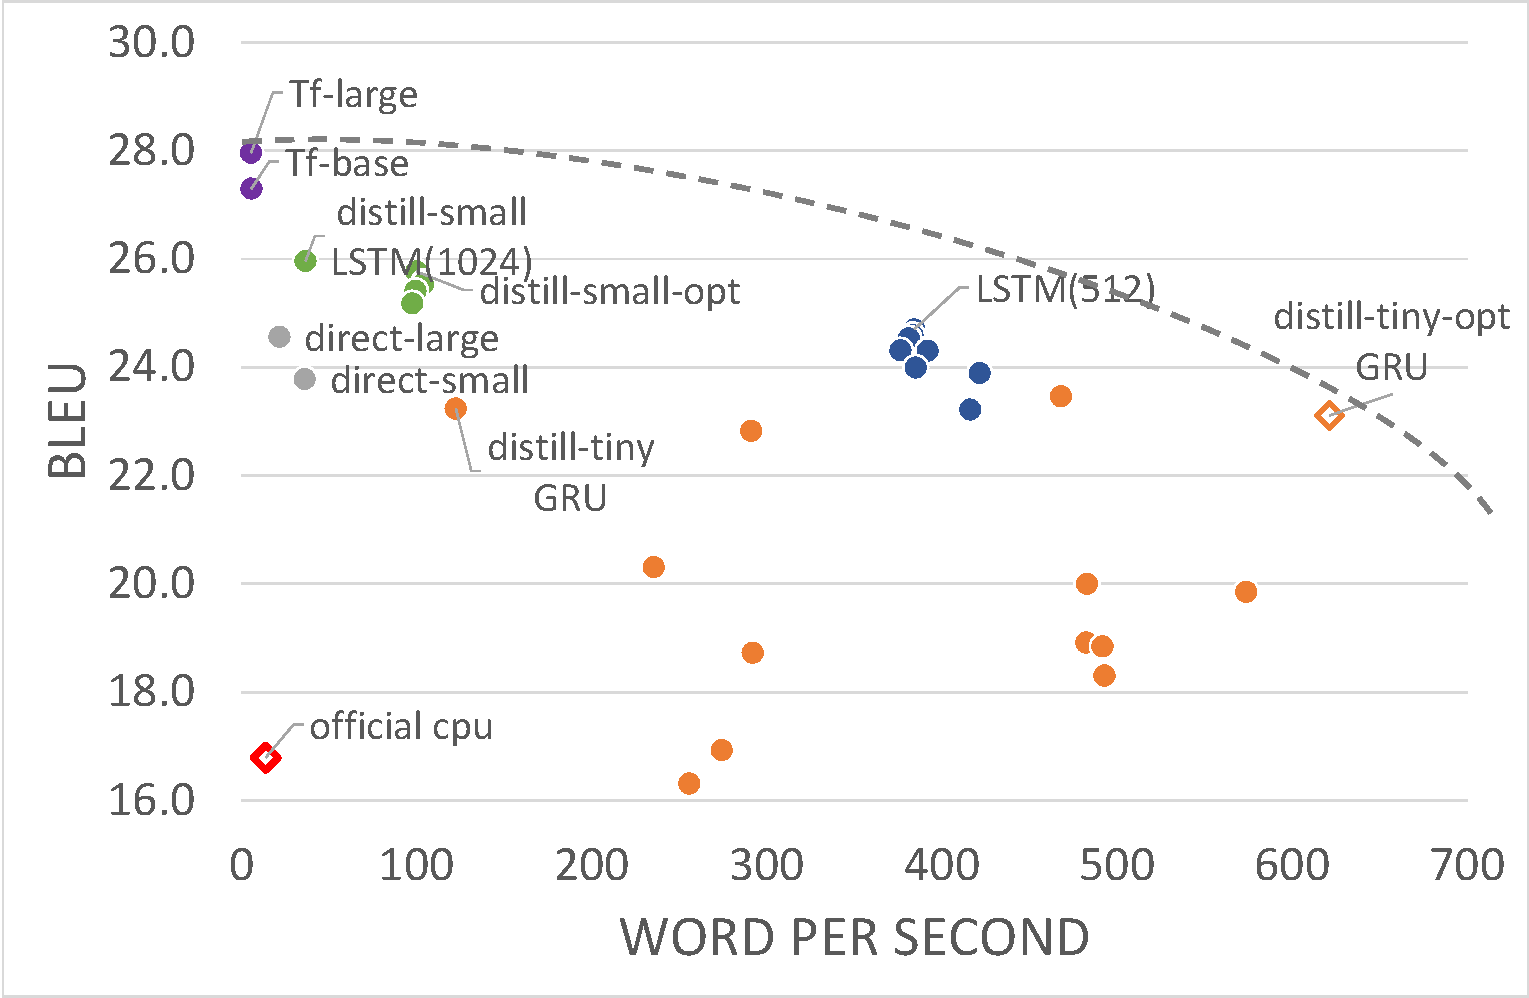
\includegraphics[width=\linewidth]{pareto.pdf}
}
\caption{Pareto on accuracy and throughput. The different models on the plot are described in the paper, the corresponding BLEU score calculated on {\it newstest2014}, and throughput in word per second measured on non dedicated M5 instances.}
\label{fig:pareto}
\end{figure}

Our experiments compare the different approaches in terms of speed and
accuracy. A meta question of this work is to decide which models
represent interesting and useful points on the Pareto curve. The main
results are described in Figure~\ref{fig:pareto}.  From these results
we highlight two models which were submitted to the shared task: Our
first system {\tt distill-small-opt} is a 2-layer LSTM network that is only
-2.19 BLEU points behind that reference transformer model, but with a
speed-up of {x18}. Our second system achieves 23.11 on
WNMT 2018 English-German {\it newstest2014} (-4.85 behind the reference
model) but with an additional decoding speed-up of {x8}.
The final model reaches 800 words/sec on the dedicated evaluation CPU hardware and is the fastest CPU model submitted.

% By combining all these techniques, we generate a large number of
% models and picked two of them presenting interesting trade-off between
% speed and quality and on the frontier of the Pareto curve (see Figure
% \ref{fig:pareto}). Our first system {\tt LSTM-opt-2} is a simple
% 2-layer LSTM network is only -2.19 points behind reference transformer
% model, with a speed-up of \textcolor{red}{x18}. Our second system
% achieves 23.11 on WNMT 2018 English-German newstest2014 (-4.85 behind
% the reference model) but with an additional decoding speed-up of
% \textcolor{red}{x6} at about 800 words/sec on the evaluation
% hardware.

We additionally report several new results about recent work in NMT
and model efficiency: (a) we show that distillation of transformer
model outperforms training result of a strong RNN model - extending
findings of \newcite{DBLP:journals/corr/CregoS16} who reported that
student models could outperform their teacher for reference RNN-based
model. (b) we show that distillation from a transformer neural network
to a simple RNN neural network is efficient, (c) we compare
quantitatively different quantizations, and (b) we give an improved
algorithm to dynamically select  target vocabulary for a given batch.
Finally, we also report several complementary experiments that
resulted in  systems inside of the pareto convex border. For instance, we
compare using 8-bit quantization to 16-bit quantization.

%\begin{table}[]
%\centering
%\begin{tabular}{lccccrr}
%\toprule
%Trans.                    & \multicolumn{1}{l}{\(\displaystyle N \)} & \multicolumn{1}{l}{\(\displaystyle d \)} & \multicolumn{1}{l}{\(\displaystyle d_{ff} \)} & \multicolumn{1}{l}{\(\displaystyle h \)} & \multicolumn{1}{l}{N2014} & \multicolumn{1}{l}{N2015} \\
%
%\midrule
% Base  & 6                     & 512                        & 2048                  & 8                        & 27.30                            & 29.36                            \\
% Large & 6                     & 512                        & 4096                  & 8                        & 27.96                            & 29.95                            \\
%\bottomrule
%\end{tabular}
%\caption{\small Evaluation of base and large transformer teacher model on Newstest 2014 and 2015.}
%\label{table:transformer}
%\end{table}

\section{Training and Distillation}

% \subsection{Data}
% \label{data}

Following the shared task setup, we use the data set provided by WNMT
2018, which is a preprocessed and tokenized version of WMT 2014 on
English-German
translation\footnote{\url{https://nlp.stanford.edu/projects/nmt/}}. The
training data contains about 4.5M sentence pairs. We use {\it newstest2013}
as the validation set and {\it newstest2014} and {\it newstest2015} as the testing
sets. Before training, we trained a 32K joint byte-pair encoding (BPE)
to preprocess the data \cite{sennrich2015neural}. Hence, the generated
subword vocabulary is less than 40K word pieces. We limit the sentence
length to 100 based on BPE preprocessing in both source and target
side (excluding only $0.31\%$ of the training corpus). After decoding,
we remove the BPE joiners and evaluate the tokenized output with
multi-bleu.perl \cite{koehn2007moses}.

\subsection{Teacher Model: Transformer}
\label{transformer}

Transformer networks \cite{vaswani2017attention} are the current state-of-the art in many machine translation tasks \cite{DBLP:journals/corr/abs-1803-02155}.
%For our base teacher model, we train a transformer NMT system \cite{vaswani2017attention}.
%Unlike standard sequence-to-sequence models, transformer does not use recurrent or convolution networks.
The network directly models the representations of each sentence
with a self-attention mechanism.  Hence much longer term dependencies
can be learned, which is especially important for language pairs like
English-German.
%It currently achieves state-of-art results for machine translation \cite{DBLP:journals/corr/abs-1803-02155}.
In addition, transformer allows to easily parallelise the MLE training process across multiple GPUs.
However, a large number of parameters are needed by the network to obtain its best performance.
In order to reduce the model size, we applied knowledge distillation, a technique that has proven successful for reducing the size of neural models. We considered the transformer network as our teacher network.

%Due to their current effectiveness, it would be tempting to use the
%transformer architecture directly for our final system (and other
%submissions took this approach). However we decided not to use this
%strategy. For one transformer networks still require a large number of
%parameters and also large memory to achieve the best
%performance. Additionally some of the training benefits of transformer
%are less apparent in auto-regressive inference.

%As a result, the parallelizable training, the flexibility in modeling
%both long-range/local dependencies, and the state-of-the-art
%performance make this architecture suitable to act as our teacher
%system.

We used \textit{OpenNMT-tf}\footnote{\url{https://github.com/OpenNMT/OpenNMT-tf}}
to train two transformer based systems: base and large described in
Table \ref{table:config} with their evaluation in Table \ref{table:score}. For both, the
learning rate is set to 2.0 and warmup steps 8000, we average the last
8 checkpoints to get the final model. Our baseline system outperforms
the provided baseline Sockeye model by +0.37 BLEU on {\it newstest2014}.

\subsection{Distillation to RNN}
\label{distill}

To train our smaller student system, we follow the sequence-level
knowledge distillation approach described by
\newcite{distillation}. First, we build the full transformer as
above. Next, we use the teacher system to retranslate all the training
source sentences to generate a simplified target sentences set.  Then,
we use this simplified corpus (original source and newly generated
target) to train a student system.  The student system can be assigned
with smaller network size, in our case an RNN-based
sequence-to-sequence models similar to \newcite{bahdanau2014neural}

Results from \newcite{DBLP:journals/corr/CregoS16} show that the
distillation process not only improves throughput of the student
models and reduce their size, but can also improve the translation
quality if the width of the network is not reduced too much. Also,
these distilled systems have the interesting feature that they
performed almost identically when reducing beam search size $K$ from
$K=5$ to $K=2$. Seemingly the smaller model learns from more consistent
translations and can produce effective results with simpler syntactic
structure and even word choices. One major question here was to find
out whether cross-class distillation works as well, here from an
transformer model to student RNN model.

Our student NMT system follows the standard architecture of
~\newcite{luong-pham-manning:2015:EMNLP}. It is implemented as an
encoder-decoder network with multiple layers of a RNN with Long
Short-Term Memory hidden \cite{Hochreiter:1997:LSM:1246443.1246450} units and attentional architecture. Full details of the
\textit{OpenNMT}\footnote{\url{https://github.com/OpenNMT/OpenNMT}}
system are given in \newcite{KleinKDSR17}.
%Additional details are given in \cite{DBLP:journals/corr/CregoKKRYSABCDE16}.

% We proved it was the case, since the best distilled system
% outperforms a larger model trained with the original data.

\subsection{Model Analysis}
\label{seq2seq}


\begin{figure}
\scalebox{0.85}{
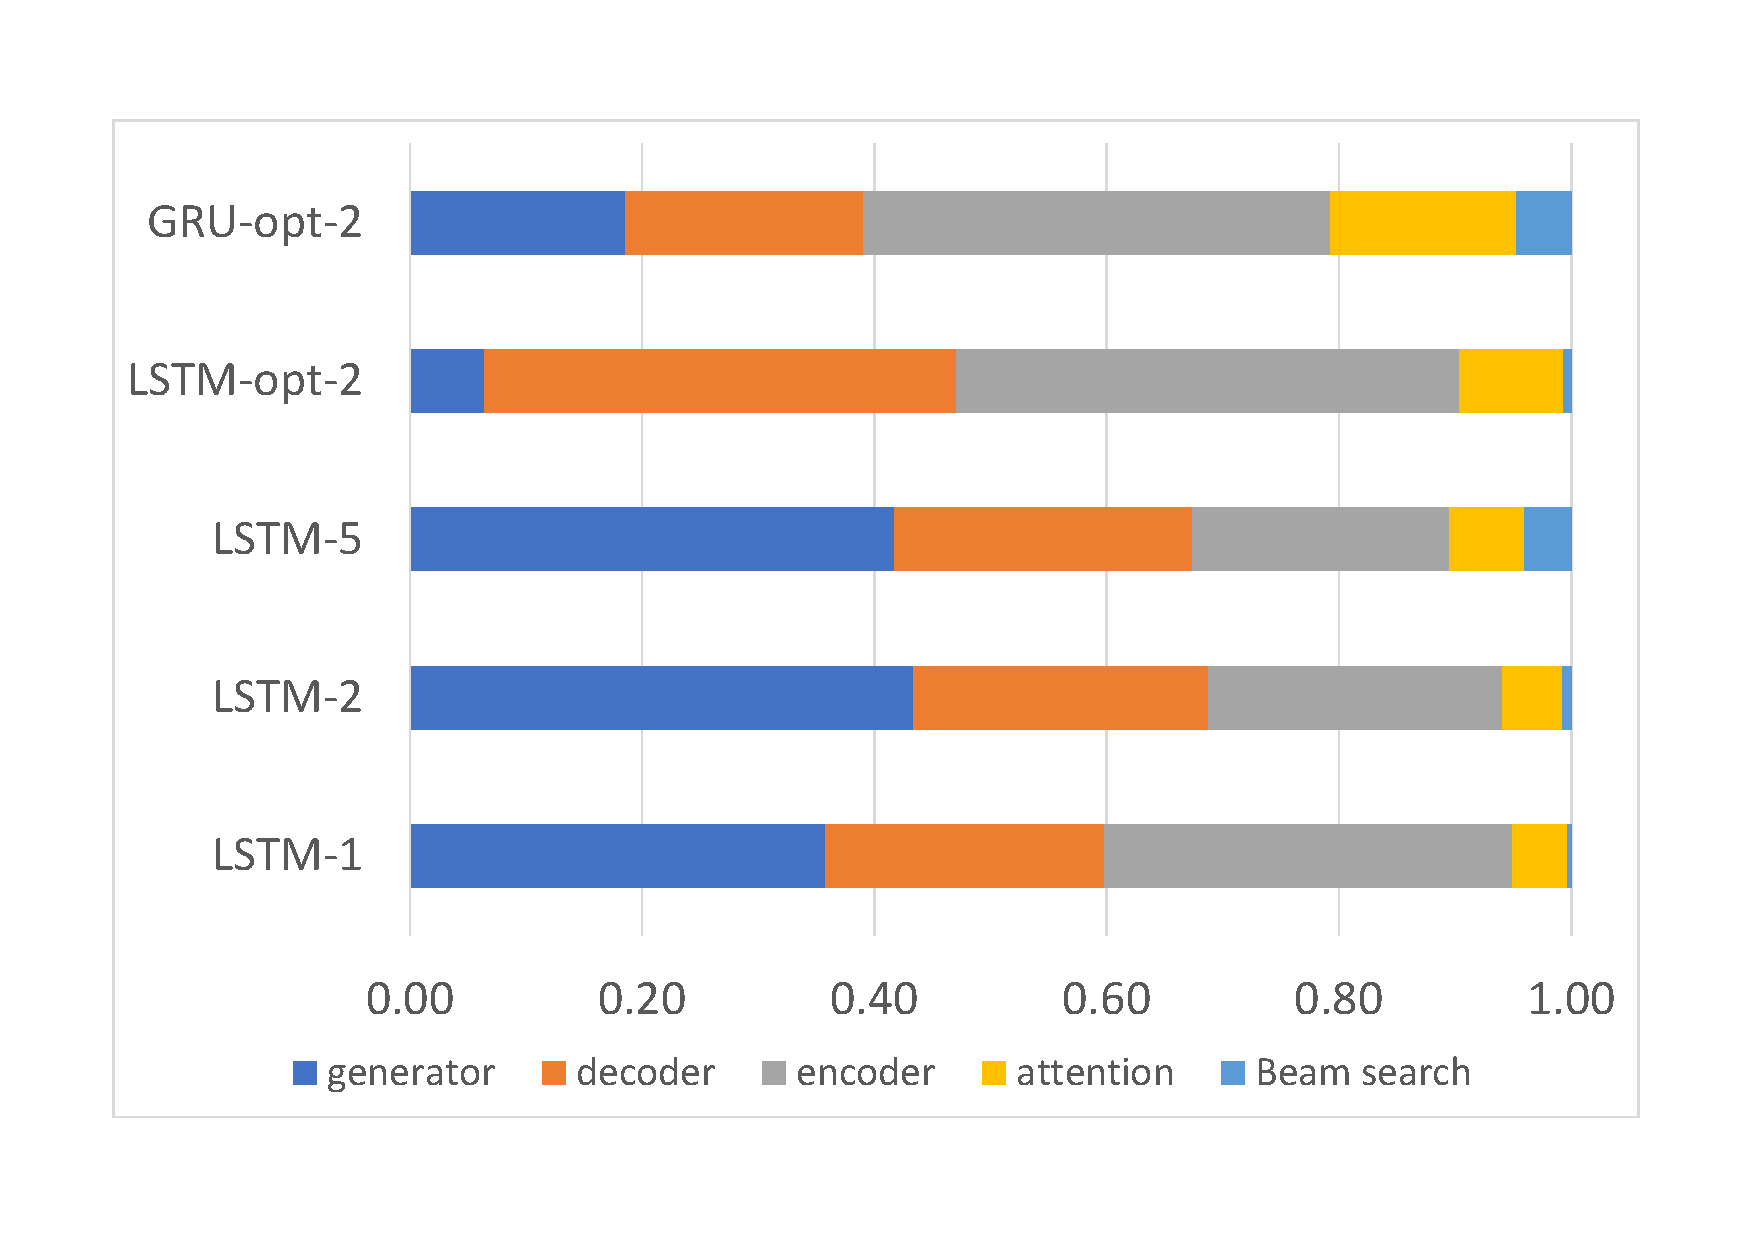
\includegraphics[width=\linewidth]{decoder.pdf}
}
\scalebox{0.85}{
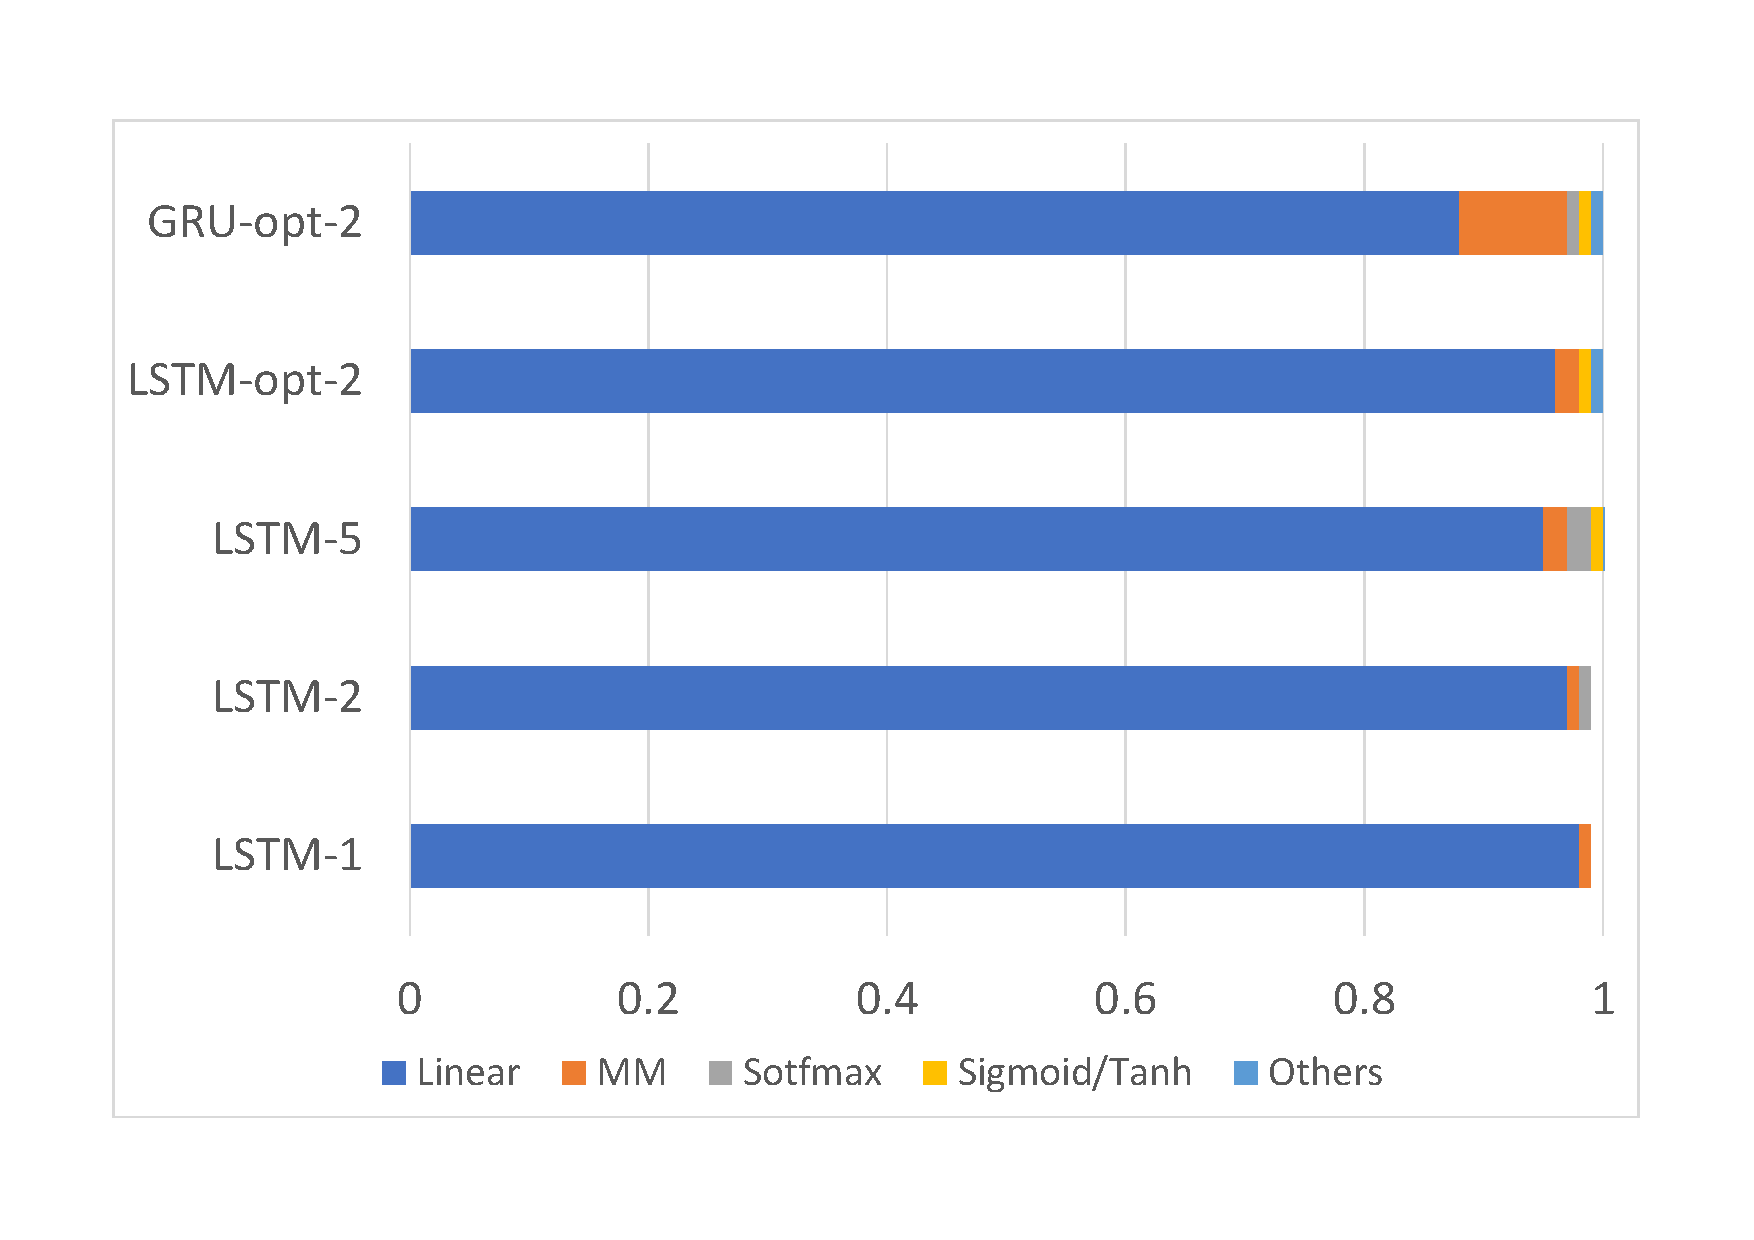
\includegraphics[width=\linewidth]{decoder_linear.pdf}
}
\caption{\small Profiling of the throughput during inference on {\it newstest2014}. Each line is a different system. The {\tt small-1,2,5} are distilled systems with respective beam size of 1, 2, 5. {\tt distill-tiny-opt} and {\tt distill-small-opt} are the final systems. The total decoding time for each of these systems (in seconds) are from top to bottom: 60, 464, 754, 662 and 629. The top table show the distribution of time per component of the network, while the bottom table show the distribution of time for network operators.}
\label{fig:decoding_cost}
\end{figure}


Profiling of the throughput of our student system, before
and after further optimizations, is presented in Figure~\ref{fig:decoding_cost}. Here we compare along two splits,
the components of the system: encoder, decoder, attention, word generation, and beam search; and model components: linear, MM (matrix multiply, primarily in attention), softmax, activations, and others.
From this analysis we gather the following facts:

\begin{itemize}
\item The most costly part of the inference is the generator, that is the final Linear layer feeding Softmax with weights corresponding to each single vocab of the target language. This is by far the largest matrix multiplication of the system: $(B,W) * (W,V)$ (with $B$ being the batch*beam size, $W$ the width of the network, and $V$ the size of the vocabulary).
\item Although the cost of the encoder for beam size 1 is higher than the decoder, the decoder cost - including generator and attention model - grows linearly with the beam size.
\item The most costly operation are the Linear matrix-vector multiplies in the RNNs and generator,
  contributing more 95\% of the complete processing time.
\end{itemize}

For these observations, it is obvious that we need to optimize the
efficiency of linear matrix-vector operation, reduce the amount
required, and have a special focus on the generation layer.

These observations led us to several further model experiments.  First
we tried different model combination based on a ``fat encoder, thin
decoder'' spirit: ie. increasing if necessary the number of operations
in the encoder part if we can in parallel reduce the number of
operations in the decoder. Second, we experimented with replacing LSTM
cell with GRU cells \cite{DBLP:journals/corr/ChoMGBSB14}. Indeed LSTM
cells have 4 gates while GRU cells only 3, so potentially leading to a
25\% improvement in speed with similar performance can be
reached. Note though, that we found GRU requires more care in optimization
while a naive SGD optimization is generally sufficient for
LSTM-RNN training.

%The same profiling on the submitted system lead to additional findings on which we elaborate in the conclusion.

\section{Inference Optimizations}

%introduction is analysis of profiling
%=> fat encoder, thin decoder

% model is Microsoft paper

% no FC -> no convergence?
% full quantized graph
% sigmoid quantizatgio

\subsection{Implementation: CTranslate}

We begin with a custom RNN decoder.  CTranslate is the open-source
inference engine for OpenNMT models (designed for Lua Torch).  The
code is implemented in raw C++ with minimal dependencies using the
popular Eigen linear algebra library. CTranslate's goal is to offer a
lightweight and embeddable solution for executing models. It benefits
from Eigen efficiency and is about 20\% faster than a Torch
application using Intel MKL. Additionally, the use of C++ over a
garbage-collected language ensures a predictable and reduced memory
usage. All additional optimizations are built on top of this library.


\subsection{Generator Vocabulary Reduction}
% find reference paper
% our contribution to extend n-gram level

As seen in the last section, the word generation matrix operations and softmax require significant time. This time is scaling linearly with the effective target language vocabulary, which starts at 40K.

There has been significant work in reducing this cost. We start with the word alignment method, presented in \newcite{shi2017speeding}, which uses alignments computed on the training corpus and for each sentence, it selects target words aligned to each source word. Hence building a reduced vocabulary of target words to be used when translating a source sentence.


To increase the coverage of the selected meanings without increasing the size of the mapping model, we first extract words in the target language that are unaligned - e.g. determiners when translating from English to French. We kept the 100 most frequent such words and call them $0$-gram meanings. Then we go through $1$-gram, $2$-gram, $\ldots$, $n$-gram sequences of words in the source sentence. For each source sequence, we consider its $N$-best translation hypotheses. All target words present in such $N$-best hypotheses are kept in the target vocabulary. To account for translation hypotheses we use a phrase table extracted from word alignments.

The method extends single word vocabulary mappings to multi-word expressions\footnote{For instance {\tt speed test} translated by {\tt test de vitesse} in French is covered by 0-grams {\tt $\varnothing\rightarrow$de}, and 1-grams {\tt speed$\rightarrow$vitesse}, {\tt test$\rightarrow$test}. However, {\tt once more} translated by {\tt \`a nouveau} will need the 2 additional meanings {\tt \`{a} } and {\tt nouveau} that are only covered when using $2$-gram meanings.}.  We have multiple criterion to extract a vocabulary map: the maximal sequence size $n$, the maximum number $N$ of translation hypotheses, the minimum frequency of a phrase pair. The efficiency of a vocabulary map can be evaluated through the coverage of the predicted meanings for a reference test set, the final translation quality and the average number of meaning per vocab, and the actual time spent in generator layer (Linear and Softmax).

Table \ref{table:ngram} compares several vocabulary maps with these
different metrics. Compared to \newcite{shi2017speeding}, our approach
with multiple $n$-gram length phrase enables better match-rate than the
$1$-gram approach (saturating the Test Coverage (TC) at 80\%).

\begin{table*}[]
\small\centering
\begin{tabular}{ccccccccc}
\toprule
\multirow{2}{*}{\begin{tabular}[c]{@{}c@{}}Max \\Sequence\end{tabular}} & \multirow{2}{*}{\begin{tabular}[c]{@{}c@{}}Min \\Freq\end{tabular}} & \multirow{2}{*}{\begin{tabular}[c]{@{}c@{}}\# \\Meaning\end{tabular}} & \multirow{2}{*}{\begin{tabular}[c]{@{}c@{}}vocab\\ per token\end{tabular}} & \multirow{2}{*}{\begin{tabular}[c]{@{}c@{}}Test\\Coverage\end{tabular}} & \multirow{2}{*}{\begin{tabular}[c]{@{}c@{}}Linear\\Time {[}s{]}\end{tabular}} & \multirow{2}{*}{\begin{tabular}[c]{@{}c@{}}SoftMax\\Time {[}s{]}\end{tabular}} & \multirow{2}{*}{File Size} & \multirow{2}{*}{BLEU} \\
\\ \midrule
 &  &  &  &  & 143.86 & 4.97 & 239M & 23.24 \\
1 & 1 & 50 & 2 & 30\% & 3.78 & 0.11 & 295M & 21.98 \\
2 & 1 & 100 & 24 & 86\% & 5.97 & 0.16 & 902M & 23.13 \\
2 & 1 & 150 & 25 & 86\% & 6.63 & 0.18 & 918M & 23.16 \\
2 & 1 & 50 & 22 & 85\% & 5.34 & 0.14 & 846M & 23.09 \\
2 & 2 & 100 & 22 & 85\% & 4.08 & 0.11 & 324M & 23.02 \\
2 & 2 & 150 & 22 & 85\% & 3.95 & 0.11 & 324M & 23.02 \\
2 & 2 & 50 & 20 & 84\% & 3.95 & 0.11 & 322M & 23.03 \\
3 & 1 & 50 & 30 & 90\% & 5.23 & 0.15 & 1127M & 23.16 \\
\bottomrule
\end{tabular}
\caption{\small Evaluations of n-gram vocabulary mappings on newstest2014.}
\label{table:ngram}
\end{table*}

\subsection{Quantization}
\label{quantize}
% nothing specific but extensipon to AVX512
Another important area of optimization is the cost of linear
matrix-operations.  To speed these up, we use 16-bit signed integer
quantization method proposed in \newcite{DBLP:journals/corr/Devlin17}.
To further optimize on the AWS M5 instance used in the
competition and powered with INTEL Skylake processors, we extend the
approach to AVX2 and AVX512 SIMD instruction sets. Switching from SSE4 to AVX2, then from
AVX2 to AVX512 instructions set gave additional speed boost of
respectively $+12\%$ and $+6\%$.

\subsection{Other Experiments}
We explored several other methods which largely resulted in
negative results but could be interesting for other contexts.

\paragraph{Decrease the sentence length:}
For BPE preprocessing, we try using 64K merges which can generate shorter sentences.
The average sentence length for 32K BPE is about 29.1 and for 64K BPE, it is about 27.7 tokens. Assuming the same efficiency in the vocabulary mapping, increasing the size of the vocabulary could therefore have gain about 5\% additional speed-up just by the reduction of the sentence length. However, the tradeoff here was not clearly a win.

 \paragraph{8-bit quantization:}
To reduce further the system size, we also considered use of {\tt gemmlowp}\footnote{\url{https://github.com/google/gemmlowp}}. {\tt gemmlowp} is a library allowing quantization to unsigned 8 bits integer through dynamic offset/multiplier/shift parameters. Like our implementation of 16-bit quantization, the low precision is only for storing the parameters, the dot product is using larger register for accumulating intermediate result of the operation. {\tt gemmlowp} usage is for embedded application where speed but also power usage is critical. The idea was tempting, but it was not clear if such quantization schema could actually outperform quantization using SIMD extended instruction set on modern processors. We ran  comparative tests using AVX2 instructions set and found out that for multiplications of large matrixes $(20,1024) * (1024,512)$ - optimized INT16 implementation was about 3 times faster than  {\tt gemmlowp} UINT8 implementation\footnote{On Intel(R) Core(TM) i7-6850K CPU @ 3.60GHz}. Main reason being that AVX2 (and AVX512 twice faster) have a very powerful multiply and add instructions\footnote{{\tt \_mm256\_madd\_epi16} and {\tt \_mm512\_madd\_epi16}} allowing to perform in one single cycle the dot product of vectors 32*INT16 and at the same time, the pair accumulation in a vector 16*INT32.

%\paragraph{Non-recurrent architectures:}
%In the same spirit of reducing the decoder layer, \newcite{DBLP:journals/corr/Devlin17} introduces an hybrid decoder with only one RNN attentional layer followed by fully connected layers with residual connections. The author reports reaching same quality than a multiple layers RNN with attention. We tried several variants around this idea but could not reproduce the same results.
%We also tried to reduce the width of the RNN more, but impact on quality was too important.

% FC
% Justin small embedding
% dense bridge
% fatter encoder did not bring
% narrower rnn 768 did not reach same level
% BPE increase - addiotnal potential gain - diff of target sentence length
% \end{itemize}

\begin{table*}[]
\centering\small
\begin{tabular}{cll}
\hline
\multirow{2}{*}{Transformer}   & Large          & N=6, d=512, \(d_{ff}\)=4096, h=8                    \\ \cline{2-3}
                               & Base         & N=6, d=512, \(d_{ff}\)=2048, h=8                    \\ \hline
\multirow{2}{*}{direct RNN}     & Large & b-LSTM, 4 layers*1024, embed=512, optim=sgd    \\ \cline{2-3}
                               & Small & b-LSTM, 2 layers*1024, embed=512, optim=sgd    \\ \hline
\multirow{2}{*}{distilled RNN} & Small          & b-LSTM, 2 layers*1024, embed=512, optim=sgd    \\ \cline{2-3}
                               & Tiny           & GRU, enc:2, dec:1 *512, embed=256, optim=adam \\ \hline
\end{tabular}
\caption{\small Configurations for the different systems presented in the paper}
\label{table:config}
\end{table*}

%\begin{table*}[]
%\centering
%\begin{tabular}{lcccccc}
%\toprule
%     & \multicolumn{1}{l}{RNN type} & \multicolumn{1}{l}{RNN size} & \multicolumn{1}{l}{encoder layers} & \multicolumn{1}{l}{decoder layers} & \multicolumn{1}{l}{embedding size} & \multicolumn{1}{l}{optim} \\ \midrule
%LSTM & b-LSTM                         & 1024                         & 2                                  & 2                                  & 512                                & sgd                       \\
%GRU & GRU                          & 512                          & 2                                  & 1                                  & 256                                & adam                      \\
%\bottomrule
%\end{tabular}
%\caption{\small Configurations for the two student systems}
%\label{table:config}
%\end{table*}

\begin{table*}[]
\centering\small
\begin{tabular}{clcccccccc}
\hline
\multicolumn{2}{c}{\multirow{2}{*}{}}    & \multirow{2}{*}{\begin{tabular}[c]{@{}c@{}}quantize\\ runtime\end{tabular}} & \multirow{2}{*}{vmap} & \multirow{2}{*}{\begin{tabular}[c]{@{}c@{}}quantize\\ model\end{tabular}} & \multicolumn{2}{c}{\it newstest2014} & \multicolumn{2}{c}{\it newstest2015} & \multirow{2}{*}{model size} \\ \cline{6-9}
\multicolumn{2}{c}{}                     &                                                                             &                       &                                                                           & cpu time {[}s{]}     & BLEU      & cpu time {[}s{]}     & BLEU      &                             \\ \hline
\multirow{2}{*}{Transformer}
                             & Large     & -                                                                           & -                     & -                                                                         &   11279.97
                   & 27.96     &           8339.10           & 29.95     &    1.4G                         \\
& Base      & -                                                                           & -                     & -                                                                         & 10795.16
                     & 27.30     &          7511.08            & 29.36     &    1.2G                         \\ \hline
\multirow{2}{*}{direct RNN}      & Large     & -                                                                           & -                     & -                                                                         &                   2859.57   & 24.56     &      2073.90                & 27.24     & 618M                        \\
                             & Small     & -                                                                           & -                     & -                                                                         &     1713.54                 & 23.78     &1313.39                      & 26.37     & 416M                        \\ \hline
\multirow{6}{*}{distilled RNN}   & Small     & -                                                                           & -                     & -                                                                         & 1694.16              & 25.96     & 1300.24              & 28.62     & 416M                        \\
                             & Small-opt & Y                                                                           & Y                     & Y                                                                         & 621.17               & 25.77     & 478.08               & 28.60     & 207M                        \\
                             & Tiny      & -                                                                           & -                     & -                                                                         & 506.67               & 23.24     & 384.76               & 26.09     & 141M                        \\
                             & Tiny      & Y                                                                           & -                     & -                                                                         & 286.89               & 23.24     & 219.85               & 26.03     & 141M                        \\
                             & Tiny      & Y                                                                           & Y                     & -                                                                         & 105.80               & 23.18     & 77.10                & 25.95     & 141M                        \\
                             & Tiny-opt  & Y                                                                           & Y                     & Y                                                                         & 99.81                & 23.11     & 77.76                & 25.75     & 72M                         \\ \hline
\end{tabular}
\caption{\small Evaluations on NMT systems (the suffix "-opt" means it is the final submission)}
\label{table:score}
\end{table*}

%\begin{table*}[]
%\centering
%\begin{tabular}{lcccccccc}
%\toprule
%\multirow{2}{*}{} & \multirow{2}{*}{\begin{tabular}[c]{@{}c@{}}quantize\\ runtime\end{tabular}} & \multirow{2}{*}{vmap} & \multirow{2}{*}{\begin{tabular}[c]{@{}c@{}}quantize\\ model\end{tabular}} & \multicolumn{2}{c}{newstest2014} & \multicolumn{2}{c}{newstest2015} & \multirow{2}{*}{model size} \\ \cline{5-8}
%                  &                                                                             &                       &                                                                           & cpu time {[}s{]}     & BLEU      & cpu time {[}s{]}     & BLEU      &                             \\ \midrule
%LSTM & -                                                                           & -                     & -                                                                         & 1694.16              & 25.96     & 1300.24              & 28.62     & 416M                        \\
%LSTM-opt & Y                                                                           & Y                     & Y                                                                         & 621.17               & 25.77     & 478.08               & 28.60     & 207M                        \\
%GRU          & -                                                                           & -                     & -                                                                         & 506.67               & 23.24     & 384.76               & 26.09     & 141M                        \\
%GRU          & Y                                                                           & -                     & -                                                                         & 286.89               & 23.24     & 219.85               & 26.03     & 141M                        \\
%GRU          & Y                                                                           & Y                     & -                                                                         & 105.80               & 23.18     & 77.10                & 25.95     & 141M                        \\
%GRU-opt          & Y                                                                           & Y                     & Y                                                                         & 99.81                & 23.11     & 77.76                & 25.75     & 72M                         \\ \bottomrule
%\end{tabular}
%\caption{\small Evaluations on two student systems (the suffix "-opt" means it is the final submission)}
%\label{table:score}
%\end{table*}

\section{Results}

\begin{figure}
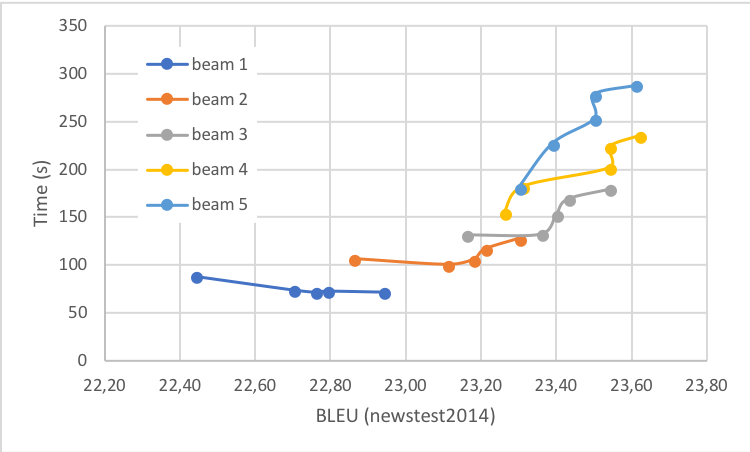
\includegraphics[width=\linewidth]{beambatch.png}
\caption{\small Evaluations on different beam size and batch size}
\label{fig:beam_batch_bleu}
\end{figure}

After tuning, we settled on two optimal NMT systems based on the
distilled training data. Table \ref{table:config}
lists the different configurations for these two systems:

\begin{itemize}
\item {\tt distill-small}, uses a bidirectional RNN with 2 LSTM layers with each hidden layer having 1024 nodes.
We use a word embedding size of 512 and set the dropout to 0.3.
The batch size is set to 64 and the default learning rate is 1.0 with sgd optimization.
\item {\tt distill-tiny}, uses  a smaller network, with GRU layers, 512 hidden size.
On the encoder side, we have 2 layers, while on the decoder side, only 1 layer is set.
We use Adam optimization with the starting learning rate 0.0002.
\end{itemize}
Both systems are trained up to 10 epochs.

Table \ref{table:score} shows our internal evaluations.
For system {\tt distill-small-opt}, the CPU time during decoding improves from 1694.16 seconds to 621.17 seconds (saving 63.3\%), with a loss of only 0.19 BLEU score, on {\it newstest2014}.
For system {\tt distill-tiny-opt}, the trends are similar.
80.3\% cpu time is saving, while only 0.13 BLEU score is lost.

We also compare the influence of quantization hyperparameters, e.g. vmap and quantize model, on tiny distilled RNN ({\tt distill-tiny}).
Quantize runtime and vmap both can save the decoding time about 50\%.
The quantized model also halves the model size.

\subsection{Beam size and Batch size}

We further test the impact on the decoding performance (BLEU) and CPU
time of different beam size and batch size on system {\tt distill-tiny-opt}.
Figure \ref{fig:beam_batch_bleu} shows for a fixed batch size, when we
increase the beam size from 1 to 3, the accuracy increases as well.
While for beam size 3, 4 and 5, there is no significant difference in
accuracy which is consistent with previous findings on distilled
system.  Interestingly, for a fixed beam size, we notice also a slight
improvement of accuracy when increasing the batch size. This is a
side-effect of the dynamic vocabulary mapping per batch.

%\begin{figure}
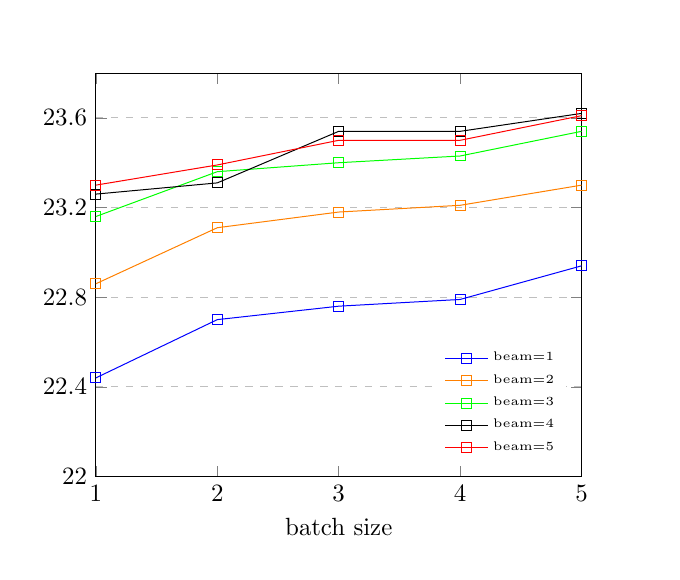
\begin{tikzpicture}
\scalebox{0.9}{
\begin{axis}[
    %title={BLEU},
    xlabel={batch size},
    %ylabel={},
    xmin=1, xmax=5,
    ymin=22, ymax=23.8,
    xtick={1,2,3,4,5},
    ytick={22.0,22.4,22.8,23.2,23.6},
    legend pos=south east,
    %legend style={font=\fontsize{4}{5}\selectfont},
    legend style={font=\tiny, draw=none},
    ymajorgrids=true,
    grid style=dashed,
]
 
\addplot[
    color=blue,
    mark=square,
    ]
    coordinates {
    (1,22.44)	(2,22.7)	(3,22.76)	(4,22.79)	(5,22.94)
    };

\addplot[
    color=orange,
    mark=square,
    ]
    coordinates {
    (1,22.86)	(2,23.11)	(3,23.18)	(4,23.21)	(5,23.3)
    };
    
\addplot[
    color=green,
    mark=square,
    ]
    coordinates {
    (1,23.16)	(2,23.36)	(3,23.4)	(4,23.43)	(5,23.54)
    };

\addplot[
    color=black,
    mark=square,
    ]
    coordinates {
    (1,23.26)	(2,23.31)	(3,23.54)	(4,23.54)	(5,23.62)
    };

\addplot[
    color=red,
    mark=square,
    ]
    coordinates {
    (1,23.3)	(2,23.39)	(3,23.5)	(4,23.5)	(5,23.61)
    };

    \legend{beam=1, beam=2, beam=3, beam=4, beam=5}
 
\end{axis}
}
\end{tikzpicture}
\caption{BLEU evaluations on different beam size and batch size}
\label{fig:beam_batch_bleu}
\end{figure}

These experiments also show that the decoding cost increases with
larger beam and batch size.  For beam size $K=1$ (in blue), we process
more sentences inside each batch and the CPU cost reduces along the
increasing of batch size.  While for the others, larger beam size and
larger batch size both cost more computational effort.

As a result,
we choose beam $K=2$ and batch $2$, balancing the performance and
computation cost.

%\begin{figure}
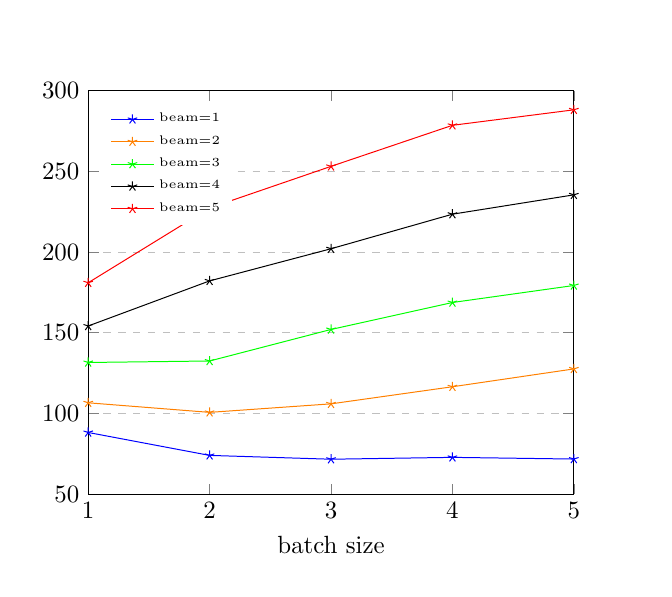
\begin{tikzpicture}
\scalebox{0.9}{
\begin{axis}[
    %title={CPU time},
    xlabel={batch size},
    %ylabel={},
    xmin=1, xmax=5,
    ymin=50, ymax=300,
    xtick={1,2,3,4,5},
    ytick={50,100,150,200,250,300},
    legend pos=north west,
    %legend style={font=\fontsize{4}{5}\selectfont},
    legend style={font=\tiny, draw=none},
    ymajorgrids=true,
    grid style=dashed,
]
 
\addplot[
    color=blue,
    mark=star,
    ]
    coordinates {
    (1,88.2)	(2,74)	(3,71.63)	(4,72.78)	(5,71.74)
    };

\addplot[
    color=orange,
    mark=star,
    ]
    coordinates {
    (1,106.59)	(2,100.66)	(3,105.94)	(4,116.53)	(5,127.58)
    };
    
\addplot[
    color=green,
    mark=star,
    ]
    coordinates {
    (1,131.57)	(2,132.49)	(3,152.02)	(4,168.73)	(5,179.27)
    };

\addplot[
    color=black,
    mark=star,
    ]
    coordinates {
    (1,154.18)	(2,182.12)	(3,202.04)	(4,223.45)	(5,235.43)
    };

\addplot[
    color=red,
    mark=star,
    ]
    coordinates {
    (1,180.97)	(2,227.26)	(3,253.09)	(4,278.52)	(5,288.11)
    };

    \legend{beam=1, beam=2, beam=3, beam=4, beam=5}
 
\end{axis}
}
\end{tikzpicture}
\caption{CPU time (seconds) on different beam size and batch size}
\label{fig:beam_batch_cpu}
\end{figure}


\subsection{Docker Image Size}

We did not invest effort into reduce image size during the preparation
of the submission. Our fastest system has a docker image of 200M for
an effective 72Mb size for the model and less than 15Mb for additional
code and resources. Post-submission, we looked at reducing this 110Mb
overhead coming from operating system and misc tools. Without huge effort - we managed to reduced
this overhead to 70Mb, and docker engineering could probably reduce even further.

\subsection{Other Engineering Considerations}

We  note that at this level of optimization, especially the use
of quantization, the speed measurement is very dependent on low level
memory management mechanisms\footnote{This effect was actually observed
during the preparation of the system: a same test could benchmark with a fluctuation
of about 10-15\% depending on the time of the day, and probable load of the
shared server hosting the virtual instance.}, and therefore on other
processes running on the same instance, especially due to the critical
importance of the L3/L4-cache shared between the different cores. In
particular, we observed that 4 parallel processes using fastest model
were only reaching a x3 speed boost. To go further on parallel
decoding, one would need to implement different ad-hoc mechanisms such as:
\begin{itemize}
\item synchronization points between
the parallel decoders to avoid waste of memory cache transfer
\item grouping of the sentences by sentence-length to optimize CPU
usage on the different cores
\end{itemize}

All the optimizations performed for that submission were focussed on the Linear layers - on the final fastest submitted system, the profile of Figure \ref{fig:decoding_cost} shows emerging room for optimization: even though the Linear share remains preponderant, some potential additional gain (between 5 and 10\%) could be achieved by focusing on the other operators.

\section{Conclusion}

% docker size => -50M
This work presents the OpenNMT submission to the 2018 Shared Task of
WNMT. We show that training with distillation using an optimized RNN
sequence-to-sequence system we can produce a very competitive
model for CPU demonstrating again the powerful effect of the distillation process and for the first time its application cross-class (Transformer$\rightarrow$RNN). This positive result implies that text simplification through distillation could be applied to more contexts.

Even though our submission was dedicated to a specific RNN-based network, most of the presented optimizations, aiming by different means to reduce and optimize the matrix multiplication operations can apply for other types of architectures.

Our final system does show an impressive increase in speed of 110x compared to the baseline system and achieves a throughput of 800 word/s on a single core which is the fastest reported so far.

\newpage

%\section*{Acknowledgments}
%
%The acknowledgments should go immediately before the references.  Do not number the acknowledgments section ({\em i.e.}, use \verb|\section*| instead of \verb|\section|). Do not include this section when submitting your paper for review.

% include your own bib file like this:
%\bibliographystyle{acl}
%\bibliography{acl2018}
\bibliography{acl2018}
\bibliographystyle{acl_natbib}

\end{document}
